\section{Estación de ITV}

\begin{frame}{Problema}
\begin{itemize}
	\item Una estación de ITV tiene $m$ líneas.
	\pause
	\item Hay $n$ vehículos que quieren repartirse entre las líneas. El vehículo $i$
	requiere un tiempo $T_i$ para ser inspeccionado.
	\pause
	\item Se pretende repartir los vehículos en las líneas de forma que la última
	inspección termine lo antes posible.
\end{itemize}
\pause

Presentaremos algoritmos con el formato:
\begin{description}
 \item[Entrada:] Vector de tiempos de los coches $T$ y número de líneas $m$
 \item[Salida:] Vector que indica en la posición $i$ a qué línea va el coche $i$-ésimo
\end{description}
\end{frame}

% TODO: descripción del greedy

% TODO: descripción del backtrack

\begin{frame}{Eficiencia}
	\begin{itemize}
		\item Problema: \textbf{Tamaño del árbol}
		\pause
		\item El tiempo crece al aumentar las \textbf{líneas} y/o los \textbf{coches}
		\pause
		\item ¿Solución para estudiar la eficiencia?
		\pause
		\item \textbf{Fijamos} el número de filas y dejamos variable el número de coches
	\end{itemize}
\end{frame}

\begin{frame}{Eficiencia-Tiempo de ejecución}
	\begin{center}
		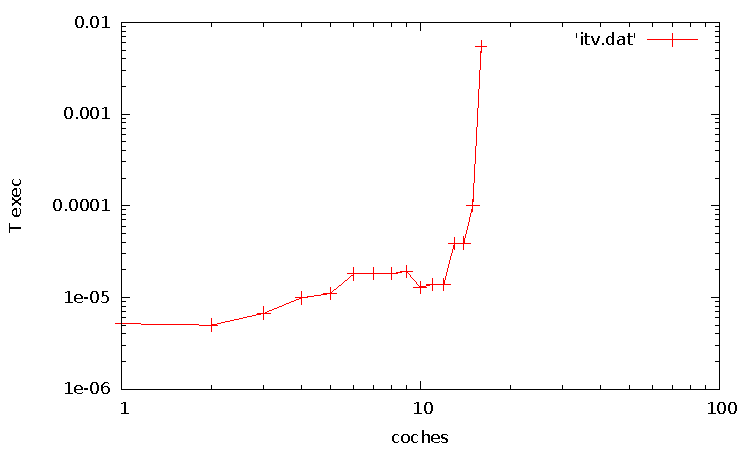
\includegraphics[width = \linewidth]{img/itvEficiencia}
	\end{center}
\end{frame}

\begin{frame}{Eficiencia-Comparación con Greedy}
	\begin{itemize}
		\item Vamos a analizar qué hemos ganado y qué perdido.
		\pause
		\item Está claro que los resultados son mejores, pero, ¿Y el tiempo?
		\pause
		\item Para $5$ líneas y $18$ coches el greedy tarda varios órdenes de magnitud menos.
		\item \textbf{¿Cuánto hemos ganado exactamente?}
		

	\end{itemize}
	\begin{center}
			\begin{tabular}{c|c|c}
				Coches	& Greedy  & Backtracking  \\ 
				17	& 190.33 &  209.09\\ 
				18	& 209.09 & 200.59
			\end{tabular}
			
	\end{center}

\end{frame}

\begin{frame}{Eficiencia-Gráfica Greedy vs Backtracking}
	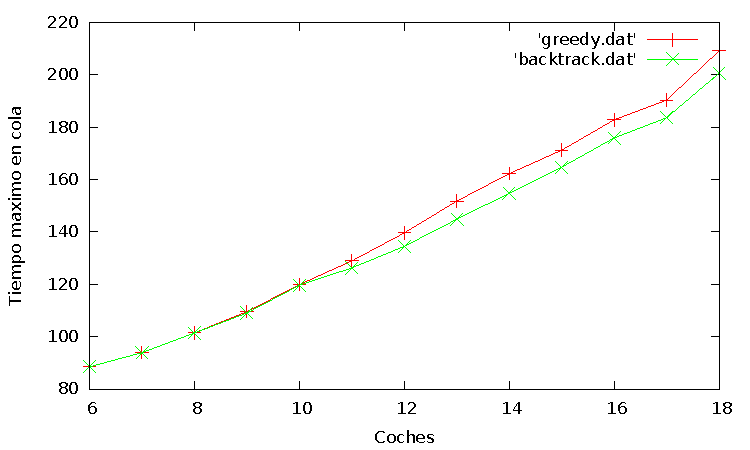
\includegraphics[width = \linewidth]{./img/comp.pdf}
\end{frame}

